\subsection{Analysis}
\label{inclusion:sec:analysis}

In this section, we evaluate the security benefits, performance, and usability
of the \excision prototype. We describe the data sets we used to train and
evaluate the system, and then present the results of the experiments.

\subsubsection{Data Collection}

\begin{table}[t]
    \centering
    \footnotesize
    \begin{tabular}{lcccc}
    \toprule
    \multirow{2}{*}{\textbf{Dataset}} & \multicolumn{2}{c}{\textbf{No. of Inclusion Sequences}} & \multicolumn{2}{c}{\textbf{No. of Terminal Domains}} \\
    \cmidrule[0.5pt](ll){2-3}
    \cmidrule[0.5pt](ll){4-5}
    & \textbf{Website Crawl} & \textbf{Extention Crawl} & \textbf{Website Crawl} & \textbf{Extension Crawl} \\
    \midrule
    Benign & 3,706,451 & 7,372 & 35,044 & 250 \\
    Malicious & 25,153 & 19 & 1,226 & 2 \\
    \bottomrule
    \end{tabular}
    \caption{Data sets used in the evaluation.}
    \label{inclusion:tab:dataset_statistics}
\end{table}


To collect inclusion sequences, we performed two separate crawls for websites
and extensions.

\paragraph{Website Crawl}

We built a crawler based on an instrumented version of
PhantomJS~\cite{phantomjs}, a scriptable open source browser based on WebKit,
and crawled the home pages of the Alexa Top 200K. We performed our data
collection from June 20th, 2014 to May 11th, 2015.

\paragraph{Extension Crawl}

To collect inclusion sequences related to extensions, we used 292 Chrome
extensions reported in prior work~\cite{www2015adinjection} that injected ads
into web pages. We chose the Alexa Top 20 shopping websites for crawling to
trigger ad injection by those 292 extensions. We built a crawler by
instrumenting Chromium~43 and collected data for a period of one week from June
16th to June 22nd, 2015.

\subsubsection{Building Labeled Datasets}
\label{inclusion:sec:building-labelled-dataset}

To classify a given inclusion sequence as benign or malicious, we trained two
hidden Markov models for benign and malicious inclusion sequences from our data
set. We labeled collected inclusion sequences as either benign or malicious
using VirusTotal~\cite{virustotal}. The malicious data set contains all
inclusion sequences where the last included resource's domain is reported
malicious by at least three out of the 62 URL scanners in VirusTotal. On the
other hand, the benign data set only contains inclusion sequences that do not
contain any domain in the entire sequence that is reported as malicious by any
URL scanner in VirusTotal. Table~\ref{inclusion:tab:dataset_statistics}
summarizes the data sets.

\subsubsection{Detection Results}
\label{inclusion:sec:detection_results}

\begin{figure}[t]
\centering
\begin{minipage}{.48\textwidth}
    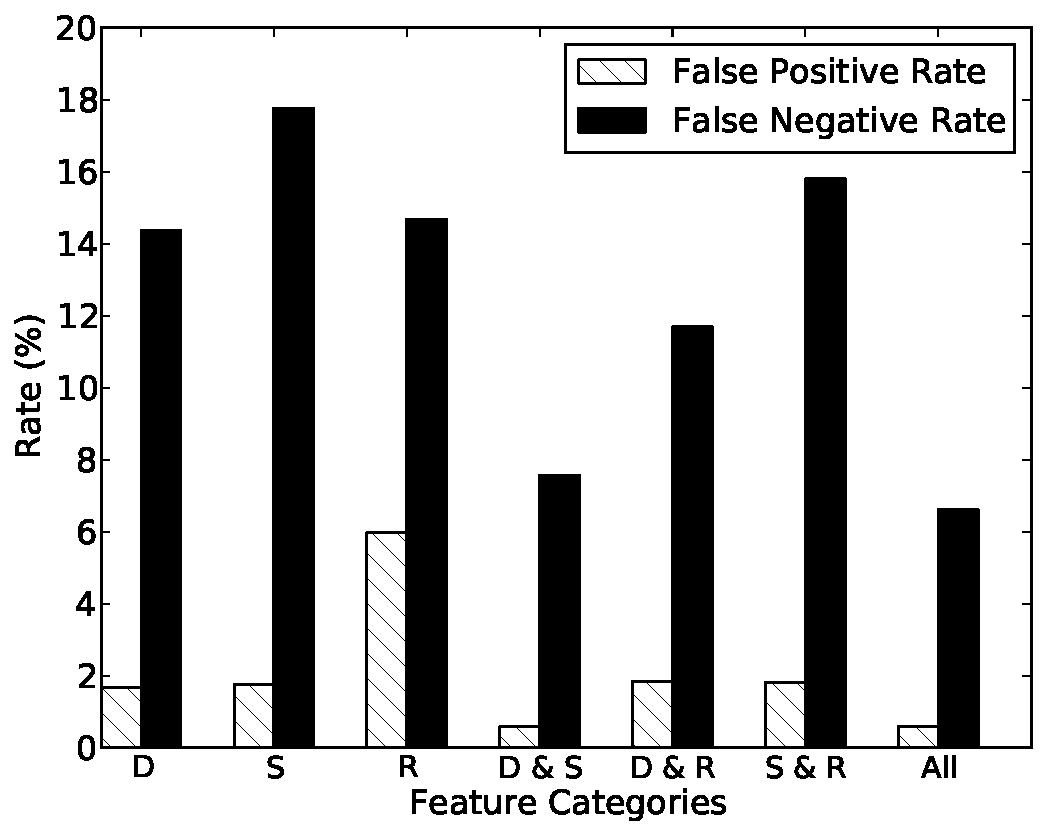
\includegraphics[width=1\textwidth,height=.8\textwidth]{inclusion/figures/detection_rate}
    \caption{Effectiveness of features for classification (D = DNS, S = String, R = Role).}
    \label{inclusion:fig:eval:detection_rate}
\end{minipage}
\hfill
\begin{minipage}{.48\textwidth}
    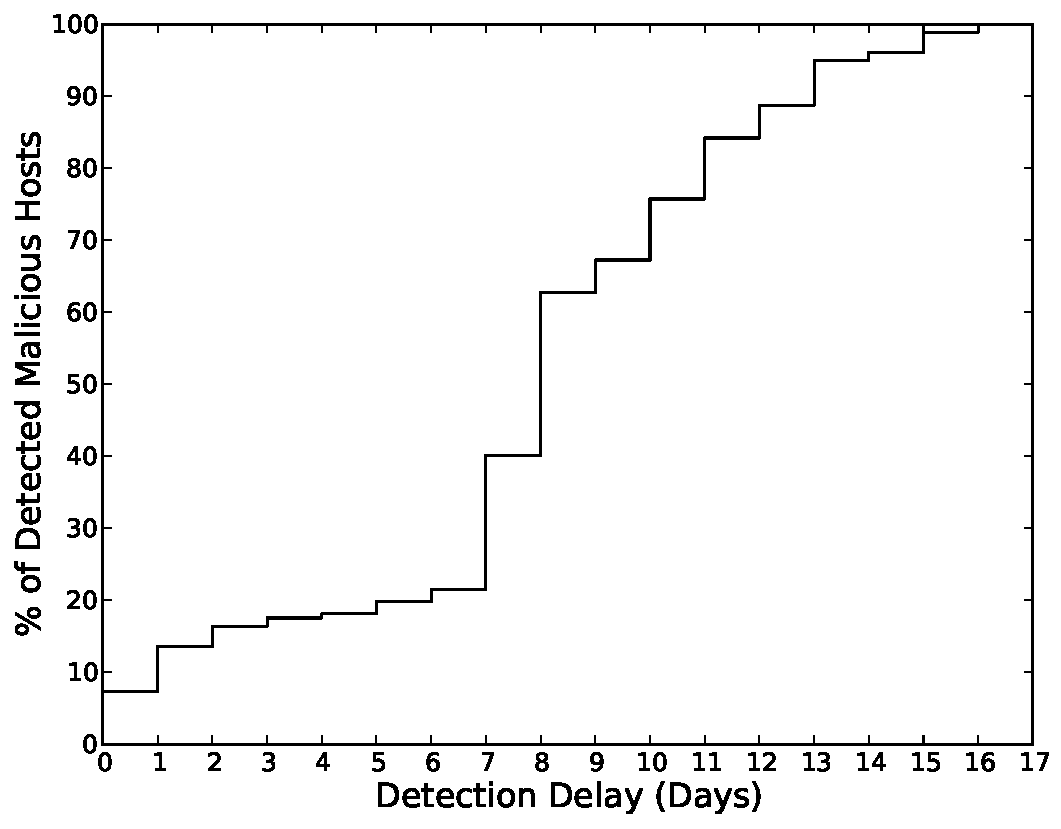
\includegraphics[width=1\textwidth,height=.8\textwidth]{inclusion/figures/early_detection}
    \caption{Early detection results.\newline}
    \label{inclusion:fig:eval:early_detection}
\end{minipage}
\end{figure}


To evaluate the accuracy of our classifier, we used 10-fold cross-validation.
When splitting the data set into training and testing sets, we made sure that
inclusion sequences with different lengths were present in both. We also ensured
that both sets contained extension-related inclusion sequences.

The results show that our classifier achieved a false positive rate of 0.59\%
and false negative rate of 6.61\% (detection rate of 93.39\%). Most of the false
positives are due to inclusion sequences that do not appear too often in the
training sets. Hence, users are unlikely to experience many false positives in a
real browsing environment (as will be shown in our usability analysis). To
quantify the contribution of different feature categories to the classification,
we trained classifiers using different combinations of feature categories and
compared the results. Figure~\ref{inclusion:fig:eval:detection_rate} shows the
false positive rate and false negative rate of every combination with a 10-fold
cross-validation training scheme.

\subsubsection{Comparison with URL Scanners}
\label{inclusion:sec:comparison}

To evaluate the ability of our system in detecting unreported suspicious
domains, we ran our classifier on inclusion sequences collected from June 1st
until July 14th, 2015. We compared our detection results with reports from URL
scanners in VirusTotal and detected 89 new suspicious domains. These domains did
not deliver malicious resources themselves, but they consistently included
resources from other domains that were flagged as malicious by URL scanners.

Furthermore, we detected 177 domains that were later reported by URL scanners
after some delay. Figure~\ref{inclusion:fig:eval:early_detection} shows the
early detection results of our system. A significant number of these domains
were not reported until some time had passed after \excision initially
identified them. For instance, nearly 78\% of the malicious domains were not
reported by any URL scanner during the first week.

\subsubsection{Performance}
\label{inclusion:sec:performance}

To assess the performance of \excision, we used Selenium WebDriver to
automatically visit the Alexa Top 1K with both original and modified Chromium
browsers. For each browser, we visited the home pages of the entire list of
websites and recorded the total elapsed time. We repeated the experiment 10
times and measured the average elapsed time. On average, \excision incurred a
12.2\% overhead on browsing time, which corresponds to a noticeable overhead
that is nevertheless acceptable for many users (see
Section~\ref{inclusion:sec:usability}).

\subsubsection{Usability}
\label{inclusion:sec:usability}

To evaluate the impact of \excision on the user's browsing experience, we
conducted the study on 10 students that self-reported as expert Internet users.
We provided each participant with a list of 50 websites that were selected
randomly from the Alexa Top 500 and then asked them to visit at least three
levels down in each website. In order to ensure that benign extensions were not
prevented from executing as expected in the presence of our system, the browser
was configured to load some popular extensions. Participants were asked to
report the number of visited pages and the number of errors they encountered

The results of the study show that out of 5,129 web pages visited by the
participants, only 83 errors were encountered and the majority of web pages
loaded correctly. Most of these errors happened due to relatively high load
times. In addition, none of the participants reported any broken extensions.
